%# Database File : Alg-Anis2ou-EpilAnis-SolSE1----
%@ Database source: Mathematics
\begin{alist}
\item Οι συντελεστές του τριωνύμου είναι $ a=1,\beta =-3 $  και $ \gamma=2 $. Η διακρίνουσα του θα ισούται με
\[ \varDelta=\beta^2-4a\gamma=(-3)^2-4\cdot1\cdot2=9-8=1>0 \]
επομένως έχει δύο άνισες ρίζες:
\[ x_{1,2}=\frac{-\beta\pm\sqrt{\varDelta}}{2a}=\frac{3\pm\sqrt{1}}{2\cdot1}=\frac{3\pm 1}{2} \]
άρα
\[ x_1=\frac{3+1}{2}=2\ \ \textrm{ή}\ \ x_2=\frac{3-1}{2}=1 \]
Τα πρόσημα του τριωνύμου φαίνονται στον παρακάτω πίνακα:
\begin{center}
\begin{tikzpicture}
\tikzset{t style/.style = {style = dashed}}
\tkzTabInit[color,lgt=3,espcl=2,colorC = \xrwma!40,
colorL = \xrwma!20,
colorV = \xrwma!40]%
{$x$ / .8,$x^2-3x+2$ /0.8}%
{$-\infty$,$1$,$2$,$+\infty$}%
\tkzTabLine{ , +, z, -, z, +, }
\end{tikzpicture}
\end{center}
\end{alist}
%# End of file Alg-Anis2ou-EpilAnis-SolSE1